\documentclass[12pt,a4paper,titlepage,twoside,numbers=noenddot,BCOR10mm]{scrreprt}
% BCOR10mm sorgt für Bindungsrand 10


%%%%%%%%%%%%%%%%%%%%%%%%%%%%%%%%%%%%%%%%%%%%%%%%%%%%%%%%%%%
% packages

% Kodierung der Eingabedateien, UTF8 erlaubt direkte Eingabe von Umlauten etc.
% Dateien sollten unter Windows als UTF-8 ohne BOM (byte order marker)
% gespeichert werde.
\usepackage[utf8]{inputenc}
\usepackage[T1]{fontenc} % richtiger Umgang / Silbentrennung von Wörtern, die Umlaute enthalten
% Neue deutsche Rechtschreibung
\usepackage[english]{babel}
\usepackage{lmodern}

% Index
\usepackage{makeidx} 

% Mathepaket für Befehle wie z.B. "gather" und vieles andere unabdingbar!
\usepackage{amsmath}
% Mathesymbole, z.B. für Mengensymbol für reelle Zahlen
\usepackage{amssymb} 

% Korrekte horizontale Trennstriche in Tabellen
\usepackage{booktabs}
% Spalten am Dezimalpunkt ausrichten
\usepackage{dcolumn}

% Bilder einbinden
\usepackage{graphicx}
% mehrere Bilder in einer Abbildung
\usepackage{subfig}

% Schönere Bildunterschriften
\captionsetup{format=hang,margin=10pt,font=small,labelfont=bf,labelsep=colon}
% Format für Caption von fortgesetzten Floats: "Abbildung ##.## (continued): ..."
\DeclareCaptionLabelFormat{continued}{#1~#2 (Fortsetzung)}
\captionsetup[ContinuedFloat]{labelformat=continued}

% Referenzen auf subfloats im Format Abb. 1 (b)
\captionsetup[subfloat]{labelformat=simple,listofformat=subsimple}
\def\thesubfigure{(\alph{subfigure})}

% Wenn z.B. mehrere Zitate in einer Klammer stehen, werden die Nummern sequentiell angeordnet
\usepackage{cite} 
% dt. Literaturverzeichnis
\usepackage{bibgerm}

% Hyperlinks auf URLs
\usepackage{url}

% Farbdefinitionen ermöglichen
\usepackage{color}

% Einheiten korrekt setzen, Doku: http://ctan.org/pkg/siunitx
% z. B. \SI{3.5}{\milli\meter} (siehe 1.1.1 im Beispieldokument)
\usepackage{siunitx} 

% fügt den 'X' für den Tabellen Aufbau hinzu. Die Spalten sind flexibel in
% ihrer Breite
%\usepackage{tabularx}
%\usepackage{multirow} %Tabellen Spalten über mehrere Spalten

% Hyperlinks in kompilierten PDF Dokumenten, vor dem Drucken die Linkfarbe
% anpassen!
\usepackage[pdftex,plainpages=false,pdfpagelabels,colorlinks=true,
            linkcolor=red, citecolor=blue]{hyperref}
            
% Titelseitenpaket (auswählen: MIT oder OHNE RWTH-Logo)
% LfB-Titelseite OHNE RWTH-Logo
%\usepackage{lfbbama}
% LfB-Titelseite MIT RWTH-Logo (erfordert unterschriebene Einverständniserklärung)
\usepackage{lfbbamarwth_EN}

%%%%%%%%%%%%%%%%%%%%%%%%%%%%%%%%%%%%%%%%%%%%%%%%%%%%%%%%%%%
\usepackage{fancyhdr} % fancy header
%Definition des styles "fancyplain". Dieser wird überall dort verwendet wo \pagestyle{fancy} oder
%\pagestyle{fancyplain} aufgerufen wird. fancyplain sorgt für Anwendung des definierten Styles selbst auf 
% Seiten, auf denen Latex normalerweise nach plain umschaltet (z.B. erste Seite eines Kapitels).

%der Parameter von z.B. \lhead in[] gibt das Aussehen für gerade der in {} für ungerade Seiten an
%\lhead[\fancyplain{}{\scshape\thepage}]{\fancyplain{}{\nouppercase{\scshape\rightmark}}}
%\chead[]{}
%\rhead[\fancyplain{}{\nouppercase{\scshape\leftmark}}]{\fancyplain{}{\scshape\thepage}}

\lhead[\fancyplain{}{\nouppercase{\scshape\leftmark}}]{}
\chead[]{}
\rhead[]{\fancyplain{}{\nouppercase{\scshape\rightmark}}}
\lfoot[\fancyplain{}{\scshape\thepage}]{}
\cfoot[]{}
\rfoot[]{\fancyplain{}{\scshape\thepage}}


%%%%%%%%%%%%%%%%%%%%%%%%%%%%%%%%%%%%%%%%%%%%%%%%%%%%%%%%%%%
%
% Abkürzungsverzeichnis
% http://my.opera.com/timomeinen/blog/show.dml/68644
%
\usepackage[english]{nomencl}
% Deutsche Überschrift
\renewcommand{\nomname}{Nomenclature and Symbols}
% Punkte zw. Abkürzung und Erklärung
\setlength{\nomlabelwidth}{.20\hsize}
\renewcommand{\nomlabel}[1]{#1 \dotfill}
% Zeilenabstände verkleinern
\setlength{\nomitemsep}{-0.05\parsep}
\makenomenclature
%
% Verwenden durch \nomenclature{SMD}{surface mounted device}
%%%%%%%%%%%%%%%%%%%%%%%%%%%%%%%%%%%%%%%%%%%%%%%%%%%%%%%%%%%

% Globaler Suchpfad für Bilder, so muss man nur den Dateinamen (ohne
% Dateierweiterung) angeben.
\graphicspath{{./images/}}  

% Gliederung bis zur subsection ins Inhaltsverzeichnis aufnehmen
\setcounter{tocdepth}{3}   
% Nummerierung der Kapitel (1, 1.1, 1.1.1, ...) bis zu subsubsection 
\setcounter{secnumdepth}{3}

% In Unterschriften direkt ohne Einrücken nach dem Label weiterschreiben
\setcapindent{0em}


%%%%%%%%%%%%%%%%%%%%%%%%%%%%%%%%%%%%%%%%%%%%%%%%%%%%%%%%%%%
% Eigene Befehlsdefinitionen
%
%%%%%%%%%%%%%%%%%%%%%%%%%%%%%%%%%%%%%%%%%%%%%%%%%%%%%%%%%%%

\makeindex


\begin{document}
\pdfbookmark[0]{Title Page}{Title Page}
%\sloppy %nur aktivieren, wenn es anders nicht geht
%%%%%%%%%%%%%%%%%%%%%%%%%%%%%%%%%%%%%%%%%%%%%%%%%%%%%%%%%%%%%%%
%
%       Titelseite und Erklärung
%
%%%%%%%%%%%%%%%%%%%%%%%%%%%%%%%%%%%%%%%%%%%%%%%%%%%%%%%%%%%%%%%
\addtolength{\topmargin}{1cm}
\pagestyle{empty}
%
% Typ der Arbeit
% Hier anpassen: Bachelorarbeit/Masterarbeit
\lfbbamatitle{Master's Thesis}                          
             {Development of an Image Processing Algorithm}      % Englischer Titel
             {Entwicklung und Implementierung eines Bildverarbeitungsalgorithmus}     % Deutscher Titel der Arbeit der Arbeit
             {Junior Mustermann}                     % Name des Studenten
             {Senior Mustermann, MSc}         		 % Betreuer
             {2019}                                  % Jahr
             {Aachen, January 16, 2019}         % Ort,Datum (Erklärung) -- Abgabedatum
             {Schlüsselwörter, durch, Kommata, getrennt} % erscheinen später in den Eigenschaften des kompilierten Dokuments

\addtolength{\topmargin}{-1cm}

\cleardoublepage
%%%%%%%%%%%%%%%%%%%%%%%%%%%%%%%%%%%%%%%%%%%%%%%%%%%%%%%%%%%%%%%%
%%
%%       Kurzfassung 
%%
%%%%%%%%%%%%%%%%%%%%%%%%%%%%%%%%%%%%%%%%%%%%%%%%%%%%%%%%%%%%%%%%
%\setcounter{page}{1}
%\pagenumbering{roman}
%%\setcounter{secnumdepth}{3} %steht doch auch schon im Header
%%\input{kurzfassung}
%\cleardoublepage

%%%%%%%%%%%%%%%%%%%%%%%%%%%%%%%%%%%%%%%%%%%%%%%%%%%%%%%%%%%%%%%%
%
%       Inhaltsverzeichnis
%
%%%%%%%%%%%%%%%%%%%%%%%%%%%%%%%%%%%%%%%%%%%%%%%%%%%%%%%%%%%%%%%
\pagenumbering{roman}
%\setcounter{page}{1}
\pagestyle{plain}
\pdfbookmark[0]{Table of Contents}{Table of Contents}
\tableofcontents
\cleardoublepage
%%%%%%%%%%%%%%%%%%%%%%%%%%%%%%%%%%%%%%%%%%%%%%%%%%%%%%%%%%%%%%%
%
%       Abbildungsverzeichnis
%
%%%%%%%%%%%%%%%%%%%%%%%%%%%%%%%%%%%%%%%%%%%%%%%%%%%%%%%%%%%%%%%
\pagestyle{empty}
\listoffigures
\addcontentsline {toc}{chapter}{List of Figures}
\cleardoublepage


%%%%%%%%%%%%%%%%%%%%%%%%%%%%%%%%%%%%%%%%%%%%%%%%%%%%%%%%%%%%%%%
\pagenumbering{arabic}
\pagestyle{fancy} %aktiviert eigenen Seitenstil

%so wird erreicht, dass keine Punkte hinter der section und chapter-Nummer gemacht werden
%Dies muss nach dem ersten Aufruf von \pagestyle{fancy} stehen
\renewcommand{\chaptermark}[1]{\markboth{\thechapter\ #1}{}}
\renewcommand{\sectionmark}[1]{\markright{\thesection\ #1}{}}

%%%%%%%%%%%%%%%%%%%%%%%%%%%%%%%%%%%%%%%%%%%%%%%%%%%%%%%%%%%%%%%
\chapter{Introduction} \label{chap:introduction}
Dies ist die Einleitung der schriftlichen Ausarbeitung.

\section{Abschnitte, Label und Referenzen} \label{sec:abschnitte}
Abschnitte werden mit dem Schlüsselwort $\backslash$section\{\} eingeleitet. Der Titel des Abschnitts steht dabei in geschweifen Klammern. Mit dem Befehl $\backslash$label\{\} können Marken im Text gesetzt werden, die mit dem Befehl $\backslash$ref\{\} referenziert werden. Der aktuelle Abschnitt befindet sich beispielsweise in Kap.~\ref{chap:introduction} und er hat die Nummer~\ref{sec:abschnitte}. Die Nummer wird automatisch erzeugt und auch ins Inhaltsverzeichnis geschrieben.

\subsection{Unterabschnitte}
gleiches Spiel jedoch mit $\backslash$subsection\{\}

Einige Zahlen mit Einheiten (hier wird automatisch ein Umbruch zwischen Zahl und Einheit verhindert):
\begin{itemize}
	\item Erdbeschleunigung: $g = \SI{9.81}{\meter\per\second\squared}$ oder auch $g = \SI{9.81}{m/s^{2}}$
    \item Lichtgeschwindigkeit: $c_0 = \SI{299792458}{\meter\per\second} = \SI{299792458}{m/s}$
\end{itemize}


\subsubsection{Noch eine Ebene tiefer...}
... kommt man mit $\backslash$subsubsection\{\}

\section{Abbildungen}
Hier einige Beispiele für Abbildungen.
\begin{figure}[htb]
	\centering
		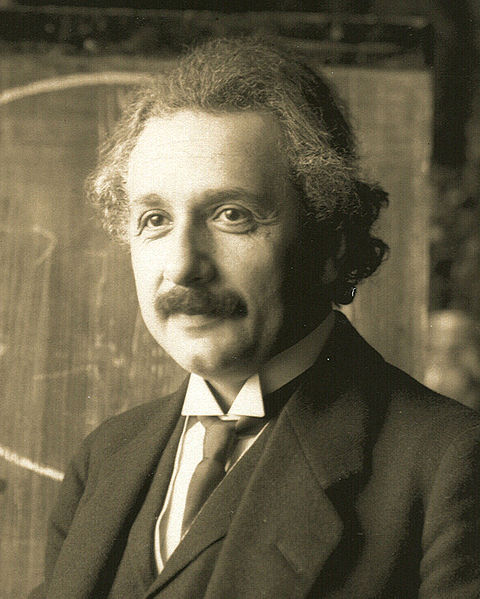
\includegraphics{Einstein}
	\caption{Ein großer Denker}
	\label{fig:Einstein}
\end{figure}


\begin{figure}[ht]
\centering
\subfloat[DER Denker schlechthin]{
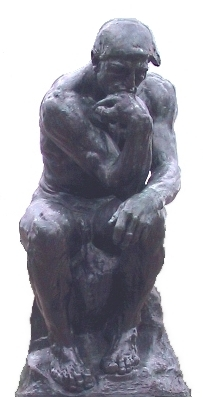
\includegraphics[width=0.275\textwidth]{Rodin-Denker-Kyoto}
\label{fig:subfig1}
} \qquad
\subfloat[noch ein Denker]{
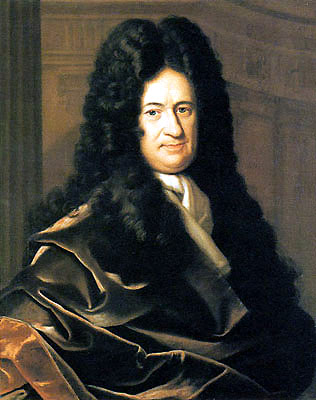
\includegraphics[width=0.4\textwidth]{Gottfried_Wilhelm_von_Leibniz}
\label{fig:subfig2}
}\\
\subfloat[und eine Denkerin]{
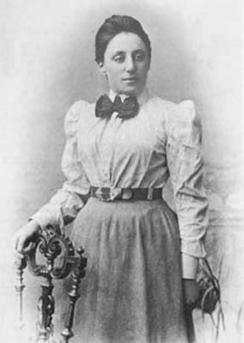
\includegraphics[width=0.4\textwidth]{Noether}
\label{fig:subfig3}
}
\caption[Kurzbeschreibung für Abbildungsindex]{Gemeinsame Beschriftung der drei Subfigures \subref{fig:subfig1}, \subref{fig:subfig2} and \subref{fig:subfig3}.
Hier auch mit längerem Text, um den Umbruch zu verdeutlichen.
Man sieht, dass der Abbildungstext links immer für sich steht.}
\label{fig:subfigureExample}
\end{figure}

\begin{figure}[ht]
\ContinuedFloat
\centering
\subfloat[DER Denker schlechthin]{
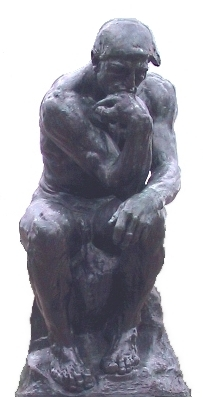
\includegraphics[width=0.275\textwidth]{Rodin-Denker-Kyoto}
\label{fig:subfig4}
} \qquad
\subfloat[noch ein Denker]{
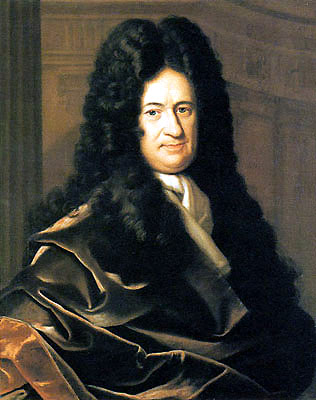
\includegraphics[width=0.4\textwidth]{Gottfried_Wilhelm_von_Leibniz}
\label{fig:subfig5}
}
\caption[Kurzbeschreibung für Abbildungsindex (Fortsetzung)]{Eine Fortsetzung der letzten Abbildung für viele Bilder.
Gemeinsame Beschriftung der zwei Subfigures \subref{fig:subfig4}, \subref{fig:subfig5}}
\label{fig:subfigureExampleCont}
\end{figure}
\cleardoublepage 

\chapter{Tables}
\label{Tabellen}
\thispagestyle{empty}

Wie erzeuge ich eine Tabelle?

Schöne Tabellen lassen sich mit dem Paket \textbf{booktabs} erzeugen, das auf die im Buchdruck unnötigen vertikalen Linien verzichtet.

% Results candidate segmentation comparison
\begin{table}[ht]\footnotesize%
\caption[]{Cell segmentation method comparison results. Performance and error measures for the segmentation of 40 test set images are provided, each method used optimized parameters.

\textit{ME}: misclassification error, \emph{MHD}: modified Hausdorff distance, \emph{OS}: over-segmentation, \emph{US}: under-segmentation, \emph{S}: sensitivity and \emph{PERF}: performance. The interquartile range (\emph{IQR}) is given for estimation of statistical dispersion of ME and MHD.}
\label{tab:candidate_segmentation_comparison}
\centering%
\begin{tabular}{p{3mm}p{4cm}*{8}{r}}
\toprule
% Header
& & \multicolumn{2}{c}{ME} & \multicolumn{2}{c}{MHD (\si{\micro\metre})} & \multicolumn{2}{c}{(\%)} & \multicolumn{2}{c}{} \\
%
\cmidrule(r){3-4} \cmidrule(r){5-6} \cmidrule(r){7-8}
%
& & \multicolumn{1}{c}{$\mu$} & \multicolumn{1}{c}{IQR} & \multicolumn{1}{c}{$\mu$} & \multicolumn{1}{c}{IQR} & \multicolumn{1}{c}{OS} & \multicolumn{1}{c}{US} & \multicolumn{1}{c}{S} & \multicolumn{1}{c}{PERF}\\
%
\midrule

                                  % method & misclass_err_mean & misclass_err_iqr & hausdorff_mean & hausdorff_iqr & oversegmentation & undersegmentation & sensitivity & performance \\
\multicolumn{10}{l}{Thresholding methods}\\
                 &  Otsu's selection method &            0.5009 &             0.68 &           10.3 &          17.6 &              0.0 &               9.4 &      0.9726 &       0.428 \\
      & Block-based selection, OD weighting &            0.3857 &             0.59 &            2.1 &           3.5 &              2.7 &               2.9 &      0.9315 &       0.503 \\
  & \textbf{Block-based, OD weighting, color distance} &            0.3929 &             0.53 &            2.8 &           4.4 &              0.0 &               4.5 &      0.9589 &       \textbf{0.533} \\
\multicolumn{10}{l}{Mean shift methods}\\
                         &  Marker stain OD &            0.4632 &             0.78 &            0.8 &           0.5 &              4.1 &               0.0 &      0.6027 &       0.187 \\
                          & Luv color space &            0.5278 &             0.79 &            2.2 &           2.7 &             12.3 &               0.0 &      0.7808 &       0.252 \\
                                   &  L-ODM &            0.4766 &             0.65 &            6.7 &           2.1 &             63.0 &               1.4 &      0.8767 &       0.147 \\
                                    &  L-OD &            0.4353 &             0.68 &            6.0 &           2.4 &             41.1 &               2.0 &      0.8356 &       0.228 \\
\bottomrule
\end{tabular}
\end{table}


\newpage

In   diesem   Abschnitt   sollen lediglich   die   grundlegenden
Eigenschaften  der  Fouriertransformation kurz tabellarisch dargestellt werden
(Tabelle  \ref{tableeigenft}). Die  Beweise zu den Regeln und  alle  Eigenschaften
sind in \cite{Aach2005} zu finden.

\begin{table}[!h]
 \begin{center}
  \begin{tabular}{|ccc|}
 \hline
 Ortsbereich &$\circ \hspace{-0.15cm} - \hspace{-0.15cm} \bullet$& Frequenzbereich\\\hline
 \hline
 Linearit"at &&  Linearit"at \\
 $k_{1}g(x)+k_{2}f(x)$ && $k_{1}G(u)+k_{2}F(u)$ \\\hline

 Symmetrie   &&  Symmetrie \\
 $F(x)$ && $f(-u)$ \\\hline

 Ortsskalierung && reziproke\\
 && Frequenzskalierung \\
 $f(kx)$ && $\frac{1}{|k|}F(\frac{u}{k})$\\\hline

 reziproke&&\\
 Ortsskalierung && Frequenzskalierung \\
 $\frac{1}{|k|}f(\frac{x}{k})$ && $F(ku)$\\\hline

 Ortsverschiebung && Phasenverschiebung \\
 $f(x-x_{0})$ && $F(u) e^{ -j 2 \pi u x_{0} }$\\\hline

 Modulation && Frequenzverschiebung \\
 $f(x) e^{ -j 2 \pi x u_{0} }$ && $F(u-u_{0})$\\\hline

 gerade Funktion && reelle Funktion \\
 $f_{g}(x)$ && $F_{g}(u)=R_{g}(u)$\\\hline

 ungerade Funktion && imagin"are Funktion \\
 $f_{u}(u)$ && $F_{u}(u)=jI_{u}(u)$\\\hline

 reelle Funktion && gerader Realteil,\\
 && ungerader Imagin"arteil \\
 $f(x)=f_{r}(u)$ && $F(u)=R_{g}(u)+j I_{u}(u)$\\\hline

 imagin"are Funktion && ungerader Realteil, \\
 && gerader Imagin"arteil \\
 $f(x)=j f_{i}(u)$ && $F(u)=R_{u}(u)+j I_{g}(u)$\\\hline

  \end{tabular}
 \end{center}
 \caption[Wichtige Eigenschaften der Fouriertransformation]{
Wichtige Eigenschaften der Fouriertransformation}
 \label{tableeigenft}
\end{table}

\cleardoublepage 

\include{formulas}
\cleardoublepage 

\chapter{Conclusions}
\label{conclusions}
\thispagestyle{empty}


\cleardoublepage 

\chapter{Outlook}
\label{outlook}
\thispagestyle{empty}


\cleardoublepage 

% Anhang
\begin{appendix}
	\chapter{Appendix}\label{cha::appendix}

\section{Formeln}
\subsection{Fast Marching}
Herleitung der Formel ...
\begin{equation}
 a^2 + b^2 = c^2
\end{equation}


	\cleardoublepage
\end{appendix}

%%%%%%%%%%%%%%%%%%%%%%%%%%%%%%%%%%%%%%%%%%%%%%%%%%%%%%%%%%%%%
%
%    Abkürzungsverzeichnis
%
%%%%%%%%%%%%%%%%%%%%%%%%%%%%%%%%%%%%%%%%%%%%%%%%%%%%%%%%%%%%%%%
%\clearpage
%\input{abkuerzungen}
%\addcontentsline {toc}{chapter}{Abkürzungsverzeichnis}
%\printnomenclature
%"%bm".nlo -s nomencl.ist -o "%bm".nls

%%%%%%%%%%%%%%%%%%%%%%%%%%%%%%%%%%%%%%%%%%%%%%%%%%%%%%%%%%%%%
%
%       Bibliographie
%
%%%%%%%%%%%%%%%%%%%%%%%%%%%%%%%%%%%%%%%%%%%%%%%%%%%%%%%%%%%%%%%
%\bibliographystyle{IEEEtran}
%\bibliography{literatur}

\clearpage

\bibliographystyle{IEEEtran}
% \addcontentsline {toc}{chapter}{Literaturverzeichnis}
\pdfbookmark[0]{Bibliography}{Bibliography}
\bibliography{literature}

\end{document}